\section{Scoring, term weighting and the vector space model}\label{ch7}

\subsection{Ranked retrieval}
Thus far, we've only considered Boolean queries, and in this sense, either a document satisfies a query or not. This methodology is good for expert users with precise understanding of their needs and the collection, but it is not good for most of the users, who are not capable of writing Boolean queries. Another problem of Boolean queries is the so-called \textit{feast or famine} problem, i.e. Boolean queries often result in either too few or too many results.

For these reasons, rather then retrieving a set of documents satisfying a query expression, in \textbf{ranked retrieval} the system reorders the top documents of a collection w.r.t. a given query. In this case, rather than a query language consisting in operators and expressions, the system deals with \textbf{free text queries}, i.e. a collection of words in human language. Notice that in the case of \textit{ranked retrieval}, the  \textit{feast or famine} issue is no longer a problem, since we just provide the top-$k$ results. 

\subsection{Parametric and zone indexes}
We have thus far viewed a document as a sequence of terms. In fact, most documents have \textbf{additional structure}. Digital documents generally encode, in machine-recognizable form, certain \textbf{metadata} associated with each document, such as its author(s), title and date of publication etc.. This metadata would generally include \textit{fields} such as the date of creation and the format of the document, as well the author and possibly the title of the document. The possible values of a field should be thought of as finite (for instance, the set of all dates of authorship). 

Consider queries of the form “find documents authored by William Shakespeare in 1601, containing the phrase \textit{alas poor Yorick}”. Query processing then consists as usual of postings intersections, except that we may merge \textbf{postings} from standard inverted as well as \textbf{parametric indexes}. There is \textbf{one} parametric index \textbf{for each field}, and it allows us to select only the documents matching a date specified in the query (in the example query above, the year 1601 is one such field value). The search engine may support querying ranges on such ordered values; to this end, a structure like a \textit{B-tree} may be used for the field’s dictionary. 

\textit{Zones} are similar to \textit{fields}, except the \textbf{contents} of a zone can be \textbf{arbitrary free text}, while a field may take on a relatively small set of values. For instance, document titles and abstracts are generally treated as zones. We may build a separate \textbf{inverted index for each zone of a document}, to support queries such as “find documents with \textit{merchant} in the title and \textit{william} in the author list and the phrase \textit{gentle rain in the body}”. This has the effect of building an index that looks like Picture \ref{zi}.

\begin{figure}[h!]
		\centering
		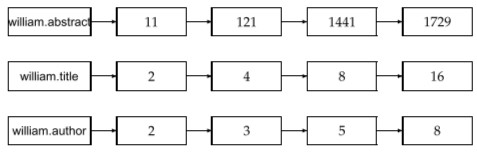
\includegraphics[scale = 2.0]{img/zone index.jpg}
		\label{zi}
        \caption{Basic zone index}
\end{figure}

We can reduce the size of the dictionary by encoding the zone in which a term occurs in the postings. In Picture \ref{zip} for instance, we show how occurrences of \textit{william} in the title and author zones of various documents are encoded. Such an encoding is useful when the size of the dictionary is a concern (because we require the dictionary to fit in main memory). 

\begin{figure}[h!]
		\centering
		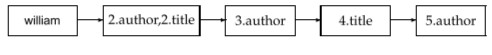
\includegraphics[scale = 2.0]{img/zone index with postings.jpg}
		\label{zip}
        \caption{Zone index in which the zone is encoded in the postings rather than the dictionary}
\end{figure}

But there is another important reason why the encoding of Figure \ref{zip} is useful: the efficient computation of scores using a technique we will call weighted zone.

\subsection{Term frequency and weighting}
Obviously, the core of the \textit{ranked retrieval} approach relies on the way we provide the \textbf{score} to each of the document, and in particular on the way we measure the importance of a query term w.r.t. the documents in the collection. 

One approach could be represented by considering the \textbf{Jaccard} coefficient between the vectors representing the query and the document. For example, if the query is "\textit{ides of march}", and the first document is "\textit{caesar died in march}" and the second document is "\textit{the long march}", then the Jaccard coefficients are:

$$
J(q,d_1) = \frac{1}{3+4-1} = \frac{1}{6}
$$

and 

$$
J(q,d_2) = \frac{1}{3+3-1} = \frac{1}{5}
$$

In this way, the result is that the second document is more relevant than the first one, but this is clearly not the case: clearly the Jaccard coefficient does not consider the \textit{term frequency}, i.e. the number of times a term occurs in a query.

Another approach is to assign the weight to be equal to the \textbf{number of occurrences} of term $t$ in document $d$. This weighting scheme is referred to as \textbf{term frequency} and is denoted $tf(t,d)$. Notice that for a document $d$, the set of weights determined by the \textit{term frequency} does not depend on the order of the terms in the document, since we only focus on the information about the number of occurrences of each term. This model is often called as \textit{bag of words} models. 

\subsubsection{Log-frequency and inverse document frequency}
Clearly, this raw definition of term frequency is not what we want from the IR system to be implemented: a document $d_1$ with 10 occurrences of a term is more relevant than a document $d_2$ with only 1 occurrence of a term, but $d_1$ is not 10 times more relevant than $d_2$. In other words, we do not want the relevance of a term to be directly proportional to its frequency.

One possible solution could be of considering the \textbf{log-frequency}, i.e.:

$$
\log tf(t,d) = \begin{cases}
1 + \log_{10} tf(t,d) \quad \text{if }tf(t,d)>0\\
0 \quad \text{otherwise }
\end{cases}
$$

In this way, the score of a query-document pair is defined as:

$$
\text{score}_{\text{LOG}}(q,d) = \sum_{t \in q \cap d} (1 + \log tf(t,d))
$$

Another possible solution exploits the \textbf{document frequency} concept: the \textit{document frequency} of a term $t$ represents the number of documents in the collection that contain the term $t$. The idea when considering \textit{document frequency} is that rare terms are more informative than frequent terms, so the documents that contain these rare terms are more likely to be relevant than documents that do not. In this sense, the \textit{document frequency} is an \textbf{inverse measure} of the \textbf{informativeness} of a term $t$. Notice that, for each term $t$, $df(t) \leq N$, where $N$ is the number of documents in the collection. The way the \textit{document frequency} is used for measuring the relevance of a term $t$ is represented by the \textbf{inverse document frequency}, which is defined as:

$$
idf(t) = \log_{10}(\frac{N}{df(t)})
$$

Some notes:

\begin{itemize}
    \item the $\log_{10}$ is used as a smoothing factor for the effect of $idf$;
    \item very frequent terms have small values of $idf$;
    \item rare terms have large values of $idf$.
\end{itemize}

In this case, the score of a query-document pair is defined as:

$$
\text{score}_{\text{IDF}}(q,d) = \sum_{t \in q \cap d} idf(t) = \sum_{t \in q \cap d} \log_{10}(\frac{N}{df(t)})
$$

Notice that $idf$ alone can produce a ranking of the matching documents only for queries with at least two terms, if all the docs do not contain all query terms.

\subsubsection{tf-idf}
We now combine the definitions of term frequency and inverse document frequency, to produce a composite weight for each term in each document, the \textit{tf-idf}:

$$
\textit{tf-idf}(t,d) = tf(t,d) * idf(t)
$$

Notice that:

\begin{itemize}
    \item the weight is higher for a term that appears many times within a small number of documents;
    \item the weight is lower for a term that occurs fewer times in a document, or that occurs in many documents. The lowest weight is obtained when the term occurs in all the documents.
\end{itemize}

At this point, we may view each document as a vector with one component corresponding to each term in the dictionary, together with a weight for each component that is given by the \textit{tf-idf}; in this case, we can compute the score as:

$$
\text{score}_{\text{TF-IDF}}(q,d) = \sum_{t \in q \cap d} \textit{tf-idf}(t,d)
$$

\underline{Example}: if we consider the table of term frequencies and idf values of Picture  \ref{ex} ,the score of Doc 1 is given by:

\begin{figure}[h!]
		\centering
		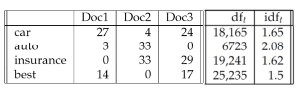
\includegraphics[scale = 2.0]{img/example tf idf.jpg}
		\label{ex}
        %\caption{Summary of compression techniques including postings}
\end{figure}

\begin{itemize}
    \item \textit{car} = $27 * 1.65 = 44.55$;
    \item \textit{insurance} = $0$;
    \item \textit{auto} = $3* 2.08 = 6.24$;
    \item \textit{best} = $14 * 1.5 = 21$
\end{itemize}

\subsection{Vector space model for scoring}
Thus far we developed the notion of a document vector that captures the relative importance of the terms in a document. The representation of a set of documents as vectors in a common vector space is known as the \textbf{vector space model} and is fundamental to a host of information retrieval operations ranging from scoring documents on a query, document classification and document clustering. The peculiarities of the documents as vectors are:

\begin{itemize}
    \item They're very \textbf{high-dimensional vectors}, i.e. they belong to an high-dimension vector space;
    \item They are very \textbf{sparse vectors}, i.e. most of the entries are equal to 0.
\end{itemize}

We recall that the goal of \textit{ranked retrieval} is to rank the documents of the collection according to their proximity to a given query. In this sense, we must provide both the vector representation for queries and the definition of proximity/similarity between vectors.

\subsubsection{Vector similarity}
We first deal with the concept of vector similarity, and we start our reasoning by considering the \textbf{euclidean distance} between two vectors. Given a document $d$ and a query $q$, the euclidean distance is defined as:

$$
dist_{\text{EUCLIDEAN}}(d,q) = \sqrt{\sum_{i = 1}^n (d_i - q_i)^2}
$$

, where $n$ is the dimensionality of the vectors. In general, the Euclidean distance is not a good measure of similarity, since it assumes large values for vectors of different lengths, i.e. the Euclidean distance of two close vectors can be very high due to their length, as represented in Picture \ref{eucl}. As we can see, the value of the Euclidean distance of $q$ and $d_2$ is very high, even if the distribution of their terms is quite similar.

\begin{figure}[h!]
		\centering
		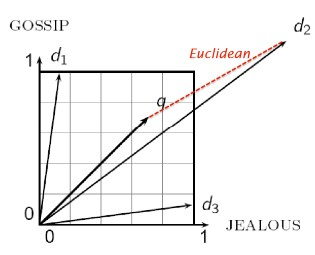
\includegraphics[scale = 2.0]{img/eucl.jpg}
		\label{eucl}
        \caption{Example of Euclidean distance}
\end{figure}

Another possible measure of the similarity of two vectors could rely on the \textbf{angle} between the vectors. In this sense, we could rank documents in increasing order of \textbf{cosine similarity} w.r.t. the query:

$$
sim_{\text{COSINE}}(\Vec{q},\Vec{d}) = \frac{\Vec{q} \cdot \Vec{d}}{|\Vec{q}||\Vec{d}|} = \frac{\sum_i q_i d_i}{\sqrt{\sum_i q_i^2} \sqrt{\sum_i d_i^2}} = \cos{\theta}
$$

, where:

\begin{itemize}
    \item $\Vec{q} \cdot \Vec{d}$ represents the \textit{dot product} between $q$ and $d$;
    \item $|\Vec{q}|$ and $|\Vec{d}|$ are the \textit{Euclidean lengths} of $\Vec{q}$ and $\Vec{d}$, and they're used to normalize the vectors $\Vec{q}$ and $\Vec{d}$ to unit vectors $\Vec{q} / |\Vec{q}|$ and $\Vec{d} / |\Vec{d}|$. In this way, long and short documents have now comparable weights.
\end{itemize}

Notice that the definition of $sim_{\text{COSINE}}$ is equal to the cosine of the angle $\theta$ between the two vectors, as showed in Picture \ref{cosine}.

\begin{figure}[h!]
		\centering
		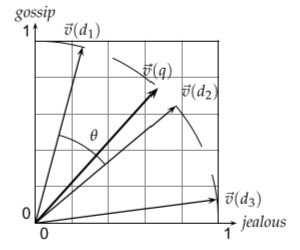
\includegraphics[scale = 2.0]{img/cosine.jpg}
		\label{cosine}
        \caption{Example of cosine similarity}
\end{figure}

What is the usage of cosine similarity?  Given a document $d$ (potentially one of the $d_i$ in the collection), consider searching for the documents in the collection most similar to $d$: we reduce the problem of finding the document(s) most similar to $d$ to that of finding the $d_i$ with the highest dot products $\Vec{d} \cdot \Vec{d_i}$. We could do this by computing the dot products between $\Vec{d}$ and each of $\Vec{d_1},..,\Vec{d_n}$, then picking off the highest resulting values.

\underline{Example}: Picture \ref{example cosine} represents the term frequencies for 4 terms in 3 different novels: in this sense, each of the novels is represented as a unit vector in three dimensions, resulting in the term frequencies weights of Picture \ref{example cosine}.

\begin{figure}[h!]
		\centering
		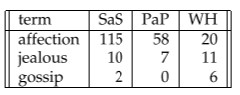
\includegraphics[scale = 2.0]{img/example cosine 1.jpg}
        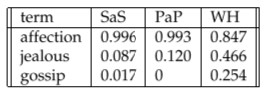
\includegraphics[scale = 2.0]{img/example cosine 2.jpg}
		\label{example cosine}
        %\caption{Example of cosine similarity}
\end{figure}

In this case, $sim_{\text{COSINE}}(\Vec{SaS}, \Vec{PaP}) = 0.996 * 0.993 + 0.087 * 0.120 + 0.017 * 0 = 0.999 $ 

Viewing a collection of $N$ documents as a collection of vectors leads to a natural view of a collection as a term-document matrix: this is an $M \times N$ matrix whose rows represent the $M$ terms of the $N$ columns, each of which corresponds to a document. As always, the terms being indexed could be stemmed before indexing;

\subsubsection{Queries as vectors}
After discussing the concept of vectors similarity, we can now notice that we can also view a query as a vector. In this way, we can assign to each document $d$ a score equal to the dot product:

$$
\text{score} = \Vec{q} \cdot \Vec{d}
$$

In other words, we can consider a query as a very short document, so we can use the cosine similarity between the query vector and a documents vector as a measure of the score of the document for that query:

$$
\text{score} = sim_{\text{COSINE}(\Vec{q}, \Vec{d})} = \frac{\Vec{q} \cdot \Vec{d}}{|\Vec{q}||\Vec{d}|}
$$

Finally, the resulting scores can be used to select the top-scoring documents for a query. However, computing the cosine similarities between the query vector and each document vector in the collection, sorting the resulting scores and selecting the top-K documents can be expensive, since a single similarity computation can entail a dot product in tens of thousands of dimensions, demanding many arithmetic operations.

\subsubsection{Computing vector scores}
In a typical setting we have a collection of documents each represented by a vector, a free text query represented by a vector, and a positive integer K: we seek the K documents of the collection with the highest vector space scores on the given query. Picture \ref{cosine score} shows the algorithm for computing vector space scores.

\begin{figure}[h!]
		\centering
		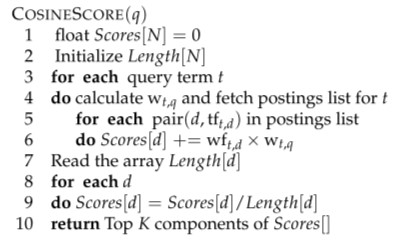
\includegraphics[scale = 2.0]{img/cosine score.jpg}
		\label{cosine score}
        \caption{Algorithm for computing vector space scores}
\end{figure}

Some notes:
\begin{itemize}
    \item the array \textit{Length} stores the lengths for each of the $N$ documents;
    \item the array \textit{Scores} stores the scores for each of the documents: when the scores are finally computed in Step 9, the top-k documents are return in Step 10;
    \item the loop in Step 3 iterates over all the query terms $t$, while in Step 5 we calculate the weight in the query vector for term $t$;
    \item Steps 6-8 update the score of each document by adding in the contribution from term $t$. This process of adding in contributions one query term at a time is sometimes known as \textit{term-at-a-time} scoring or accumulation, and the $N$ elements of the array \textit{Scores} are therefore known as \textit{accumulators}. For this purpose, it would appear necessary to store, with each postings entry, the weight $wf_{t,d}$ of term $t$ in document $d$ (we have thus far used either $tf$ or $tf-idf$ for this weight, but leave open the possibility of other functions to be developed). In fact this is wasteful, since storing this weight may require a floating point number. Two ideas help alleviate this space problem. First, if we are using inverse document frequency, we need not precompute $idf_t$; it suffices to store $N/df_t$ at the head of the postings for $t$. Second, we store the term frequency $tf_{t,d}$ for each postings entry.
\end{itemize}

\subsection{Variant tf-idf functions}
For assigning a weight for each term in each document, a number of alternatives to $tf$ and $tf-idf$ have been considered. We discuss some of the principal ones here.

\begin{figure}[h!]
		\centering
		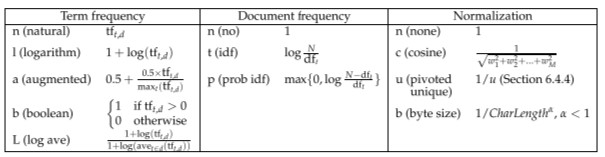
\includegraphics[scale = 2.0]{img/SMART.jpg}
		\label{SMART}
        \caption{SMART Notation for tf-idf variants}
\end{figure}

Picture \ref{SMART} lists some of the principal weighting schemes in use for each of $\Vec{d}$ and $\Vec{q}$, together with a mnemonic for representing a specific combination of weights; this system of mnemonics is sometimes called SMART notation. The mnemonic for representing a combination of weights takes the form \textit{ddd.qqq} where the first triplet gives the \textit{term weighting} of the \textit{document} vector, while the second triplet gives the \textit{weighting} in the \textit{query} vector.  The first letter in each triplet specifies the term frequency component of the weighting, the second the document frequency component, and the third the form of normalization used. 

It is quite common to apply different normalization functions to $\Vec{q}$ and $\Vec{d}$. For example, a very standard weighting scheme is \textbf{lnc.ltc}, where the document vector has log-weighted term frequency, no idf (for both effectiveness and efficiency reasons), and cosine normalization, while the query vector uses log-weighted term frequency, idf weighting, and cosine normalization.
